\begin{figure}
    \centering
    \begin{subfigure}{.3\textwidth}
        \centering
        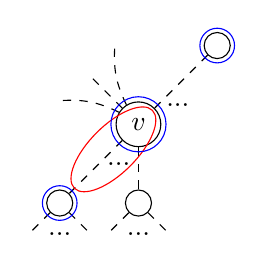
\begin{tikzpicture}
            \node[draw, circle] (a) at (1,1) {};
            \node[draw, circle] (b) at (0,0) {$v$};
            \node[draw, circle] (c) at (-1,-1) {};
            \node[draw, circle] (d) at (0,-1) {};
            \node at (-0.25,-0.5) {...};
            \node at (-1,-1.4) {...};
            \node at (0,-1.4) {...};
            \node at (0.5,0.25) {...};
    
            \draw[dashed] (a) -- (b); 
            \draw[dashed] (b) -- (c); 
            \draw[dashed] (b) -- (d); 
            \draw[dashed] (b) -- (-0.6,0.6); 
            \draw[dashed, bend left=15] (b) to (-0.3,1);
            \draw[dashed, bend right=15] (b) to (-1,0.3);
            \draw[dashed] (c) to (-1.4,-1.4);
            \draw[dashed] (c) to (-0.6,-1.4);
            \draw[dashed] (d) to (-0.4,-1.4);
            \draw[dashed] (d) to (0.4,-1.4);
    
            \draw[rotate=45, red] (-0.45, 0) ellipse (0.7 and 0.3); 
            \draw[blue] (a) circle (0.22);
            \draw[blue] (b) circle (.35);
            \draw[blue] (c) circle (.22);
    
        \end{tikzpicture}
        \caption*{A}
    \end{subfigure}
    \begin{subfigure}{.3\textwidth}
        \centering
        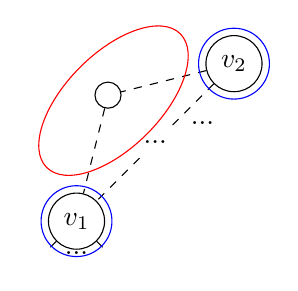
\begin{tikzpicture}
            \node[draw, circle] (a) at (1,1) {$v_2$};
            \node[draw, circle] (b) at (-0.6,0.6) {};
            \node[draw, circle] (c) at (-1,-1) {$v_1$};
    
            \node at (0.6,0.25) {...};
            \node at (0,0) {...};
            \node at (-1,-1.4) {...};
            
    
            \draw[dashed] (a) -- (b); 
            \draw[dashed] (b) -- (c); 
            \draw[dashed] (a) -- (0.2,0.2); 
            \draw[dashed] (-0.2,-0.2) -- (c); 
            
    
            \draw[dashed] (c) to (-1.4,-1.4);
            \draw[dashed] (c) to (-0.6,-1.4);
            
            \draw[rotate=45, red] (0, 0.75) ellipse (1.2 and 0.6); 
            \draw[blue] (a) circle (0.45);
            \draw[blue] (c) circle (.45);
            
        \end{tikzpicture}
        \caption*{B}
        \end{subfigure}
    \begin{subfigure}{.3\textwidth}
        \centering
        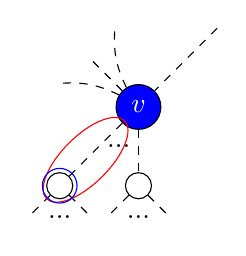
\begin{tikzpicture}
            \node[draw, circle, fill=blue] (b) at (0,0) {\textcolor{white}{$v$}};
            \node[draw, circle] (c) at (-1,-1) {};
            \node[draw, circle] (d) at (0,-1) {};
            \node at (-0.25,-0.5) {...};
            \node at (-1,-1.4) {...};
            \node at (0,-1.4) {...};
    
            \draw[dashed] (1,1) -- (b); 
            \draw[dashed] (b) -- (c); 
            \draw[dashed] (b) -- (d); 
            \draw[dashed] (b) -- (-0.6,0.6); 
            \draw[dashed, bend left=15] (b) to (-0.3,1);
            \draw[dashed, bend right=15] (b) to (-1,0.3);
            \draw[dashed] (c) to (-1.4,-1.4);
            \draw[dashed] (c) to (-0.6,-1.4);
            \draw[dashed] (d) to (-0.4,-1.4);
            \draw[dashed] (d) to (0.4,-1.4);
    
            \draw[rotate=45, red] (-0.95, 0) ellipse (0.7 and 0.3); 
            \draw[blue] (c) circle (.22);
    
        \end{tikzpicture}
        \caption*{C}
    \end{subfigure}
    \begin{subfigure}{.3\textwidth}
        \centering
        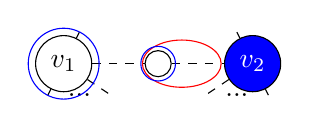
\begin{tikzpicture}
            \node[draw, circle] (a) at (-1.2,0) {$v_1$};			
            \node[draw, circle] (b) at (0,0) {};			
            \node[draw, circle, fill=blue] (c) at (1.2,0)  {\textcolor{white}{$v_2$}};
            
            \node at (-1,-0.4) {...};
            \node at (1,-0.4) {...};
    
            \draw[dashed] (a) -- (b);
            \draw[dashed] (b) -- (c);
            \draw[dashed] (a) -- (-1.4,-0.4);
            \draw[dashed] (a) -- (-0.6,-0.4);
            \draw[dashed] (a) -- (-1,0.4);
            
            \draw[dashed] (c) -- (1.4,-0.4);
            \draw[dashed] (c) -- (0.6,-0.4);
            \draw[dashed] (c) -- (1,0.4);
    
            \draw[red] (0.3, 0) ellipse (0.5 and 0.3); 
            \draw[blue] (a) circle (.45);
            \draw[blue] (b) circle (.22);
    
        \end{tikzpicture}
        \caption*{D}
    \end{subfigure}
    \begin{subfigure}{.3\textwidth}
        \centering
        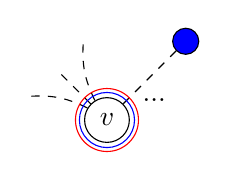
\begin{tikzpicture}
            \node[draw, circle, fill=blue] (a) at (1,1) {};
            \node[draw, circle] (b) at (0,0) {$v$};
            
            \node at (0.6,0.25) {...};
    
    
            \draw[dashed] (a) -- (b); 
            \draw[dashed] (b) -- (-0.6,0.6); 
            \draw[dashed, bend left=15] (b) to (-0.3,1);
            \draw[dashed, bend right=15] (b) to (-1,0.3);
            
            \draw[blue] (b) circle (.35);
            \draw[red] (b) circle (.4);
        \end{tikzpicture}        
        \caption*{E}
    \end{subfigure}
    \begin{subfigure}{.3\textwidth}
        \centering
        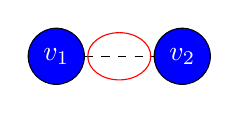
\begin{tikzpicture}
            \node[draw, circle, fill=blue] (a) at (-0.8,0) {\textcolor{white}{$v_1$}};
            \node[draw, circle, fill=blue] (b) at (0.8,0) {\textcolor{white}{$v_2$}};
        
            \draw[dashed] (a) -- (b);
            \draw[red] (0, 0) ellipse (0.4 and 0.3); 
        \end{tikzpicture}
        \vspace{1cm}
        \caption*{F}
    \end{subfigure}
    \begin{subfigure}{.3\textwidth}
    \end{subfigure}
    \begin{subfigure}{.3\textwidth}
    \end{subfigure}

    \caption{The red region shows the hiding spot of the robber. The blue circles are the cop-positions after the round. The blue verteces are places where the cops were placed in the last round and stay. Each dashed line represents a path of length $s$.}
    \label{fig:CopStragyTree}
\end{figure}